% Slides for 2025-07-29
% To create a slide, use the following:
% \begin{frame}{TITLE}
%     BODY
% \end{frame}

% To create a slide with a bullet list, use the following:
% \begin{frame}{TITLE}
%     \begin{itemize}
%         \item ITEM 1
%         \item ITEM 2
%     \end{itemize}    
% \end{frame}

% To create a slide with numbered list, use the following:
% \begin{frame}{TITLE}
%     \begin{enumerate}
%         \item ITEM 1
%         \item ITEM 2
%     \end{enumerate}
% \end{frame}

% To create a slide with a graphic:
% 1. Add the graphic to this folder (named picture.png)
% 2. Use the following:
% \begin{frame}{TITLE}
%     \centering
%     \includegraphics[height=0.7\textheight,width=0.7\textwidth,keepaspectratio]{picture.png}
% \end{frame}

% To create a slide with two columns, use the following:
% \begin{frame}{TITLE}
%     \begin{columns}
%         \begin{column}{0.5\textwidth}
%             COLUMN 1 BODY
%         \end{column}
%         \begin{column}{0.5\textwidth}
%             COLUMN 2 BODY
%         \end{column}
%     \end{columns}
% \end{frame}

\begin{frame}{Getting the Data}
    \begin{itemize}
        \item Notes from CCFRP were digitized to generate labeled data points.
        \item Calculated fish lengths were matched to ground truth measurements.
    \end{itemize}
\end{frame}

\begin{frame}{Getting Fish Lengths}
    \begin{itemize}
        \item Using annotations, depth maps, and camera intrinsics, fish lengths were calculated.
    \end{itemize}
    \vspace{1em}
    \centering
    \begin{tabular}{ccc}
        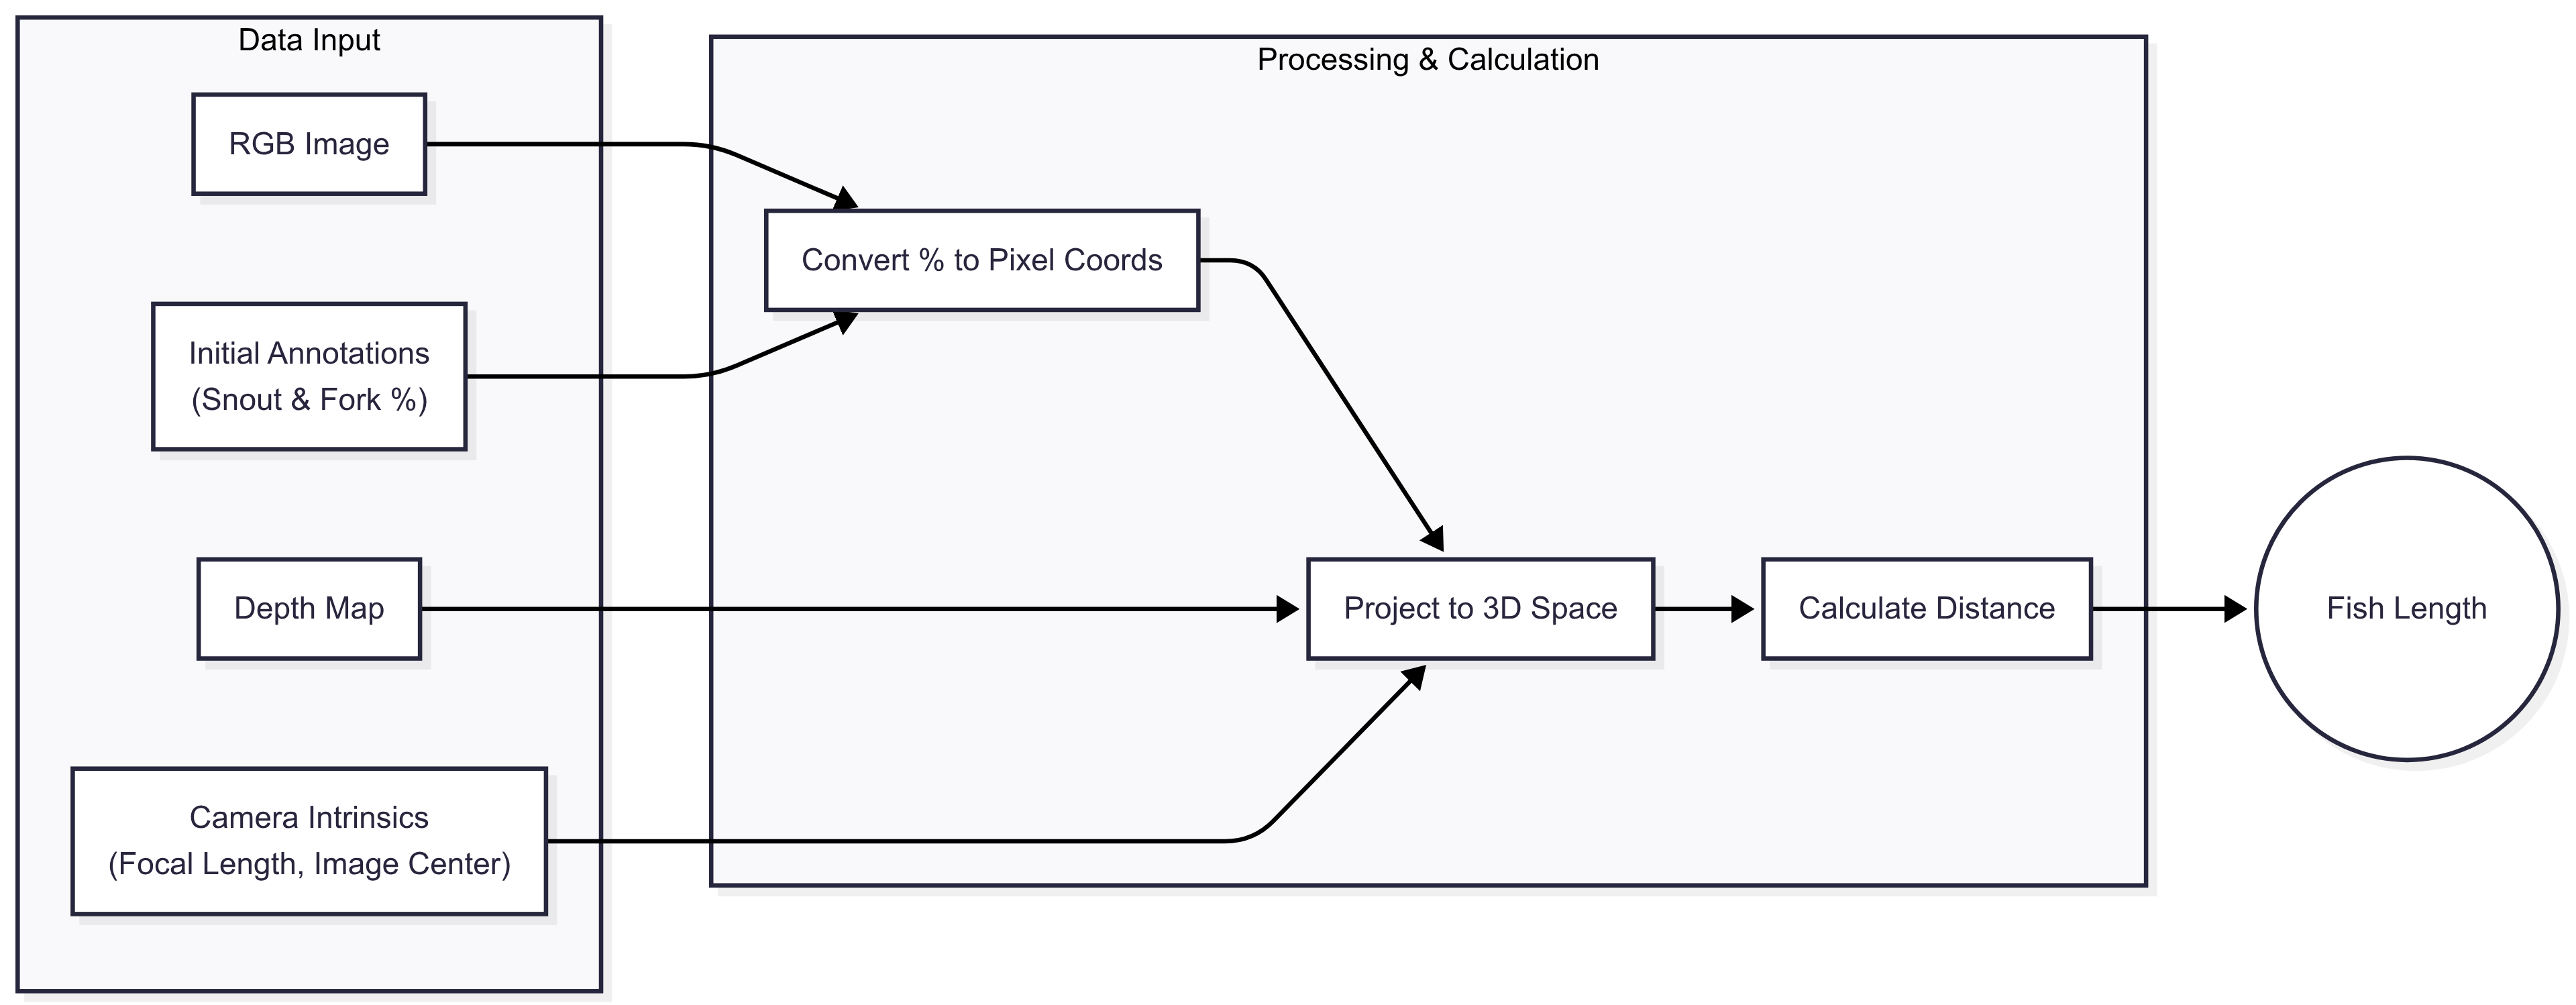
\includegraphics[width=0.8\textwidth]{images/length_measurement_pipeline.png} &
    \end{tabular}
\end{frame}

\begin{frame}{Getting Fish Lengths}
    \centering
    \begin{tabular}{ccc}
        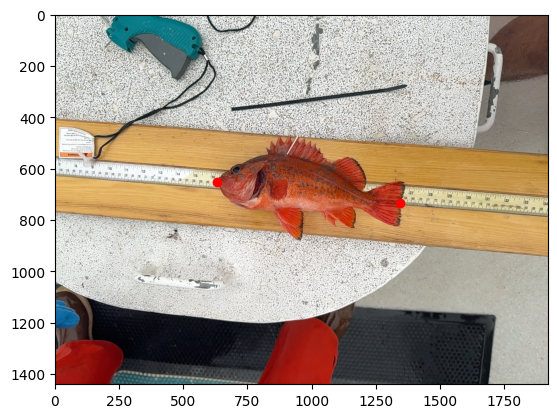
\includegraphics[width=0.3\textwidth]{images/rgb1.png} &
        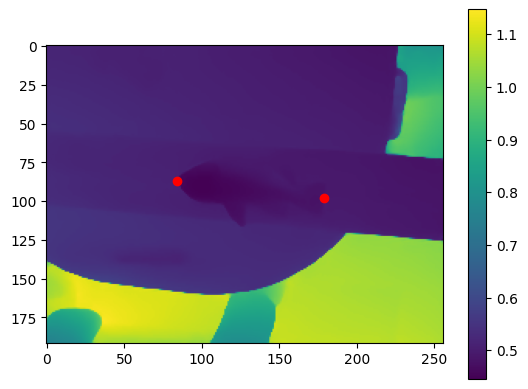
\includegraphics[width=0.3\textwidth]{images/depth1.png} &
        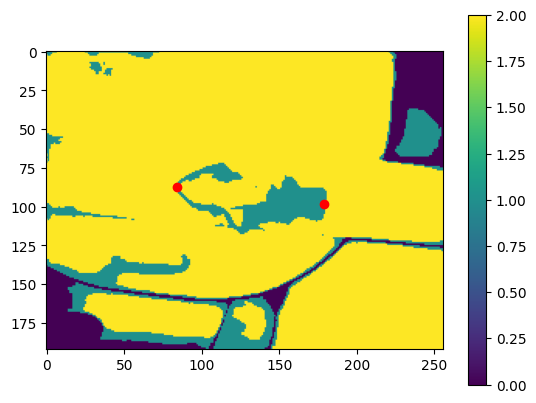
\includegraphics[width=0.3\textwidth]{images/confidence1.png} \\
        \small RGB Image & \small Depth Map & \small Confidence Map \\
    \end{tabular}
\end{frame}

\begin{frame}{Let's Look at Some Results}
    \centering
    \begin{tabular}{@{}cc@{}}
        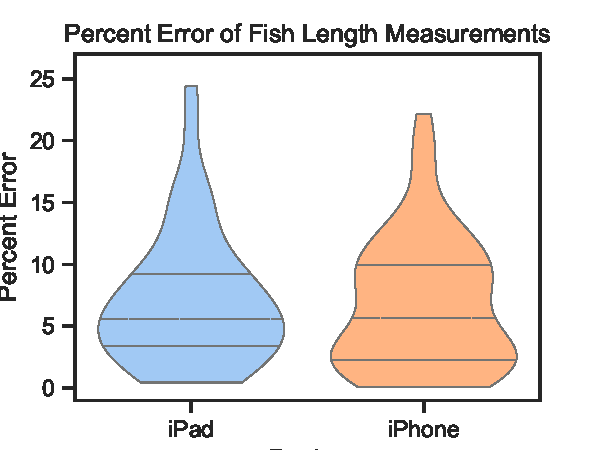
\includegraphics[width=0.3\textwidth]{images/device_error.pdf} &
        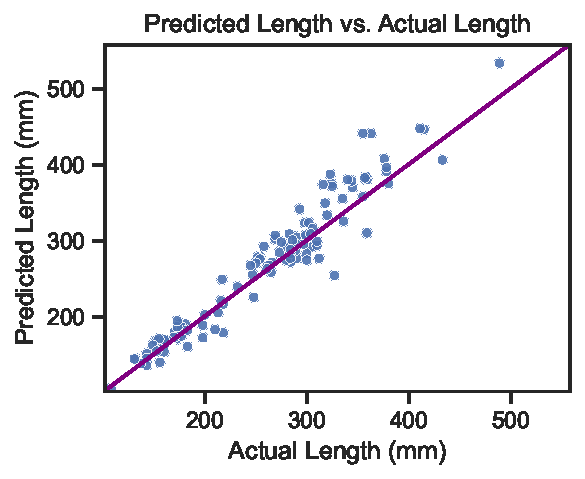
\includegraphics[width=0.3\textwidth]{images/fsm_all_scatter.pdf} \\
        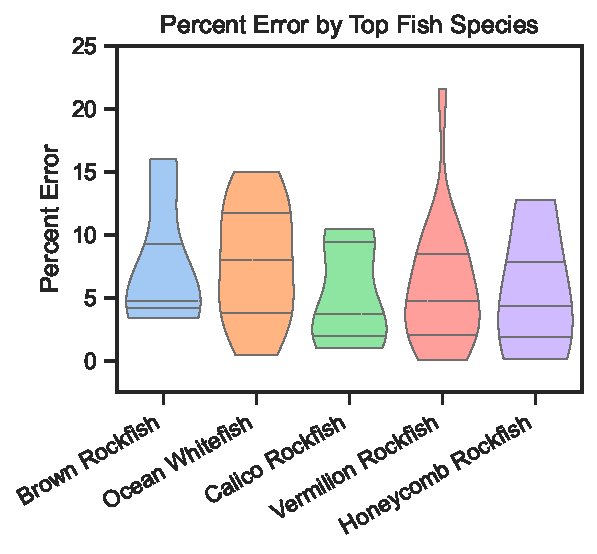
\includegraphics[width=0.3\textwidth]{images/top_species_error.pdf} &
        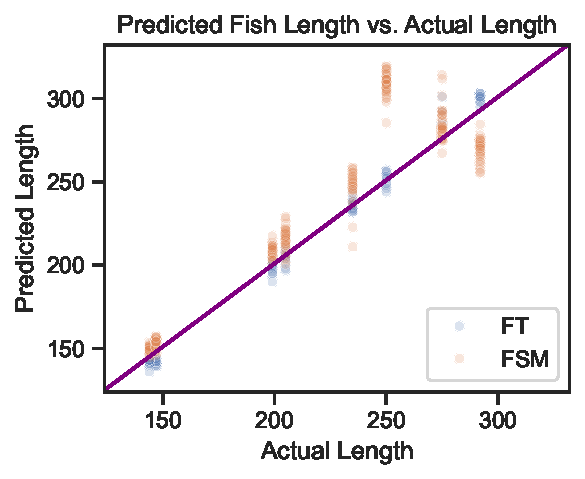
\includegraphics[width=0.3\textwidth]{images/fsm_ft_scatter.pdf} \\
    \end{tabular}
\end{frame}

\begin{frame}{Species Specific Error}
    \centering
    \begin{tabular}{ccc}
        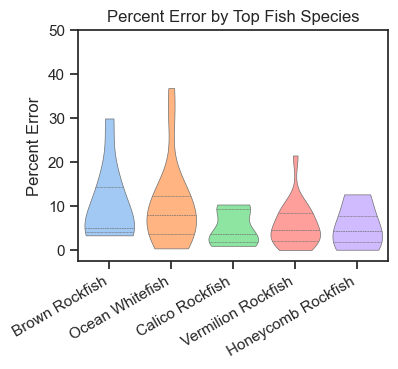
\includegraphics[width=0.45\textwidth]{images/species_plot_outdated.png} &
        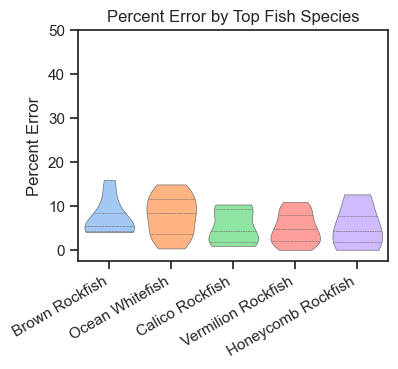
\includegraphics[width=0.45\textwidth]{images/new_species_plot_2.png} \\
        \small Figure with outliers & \small Updated Figure after correction\\
    \end{tabular}
\end{frame}

\begin{frame}{Diagnosing the Data}
    \begin{columns}[c]
        \column{0.66\textwidth}
        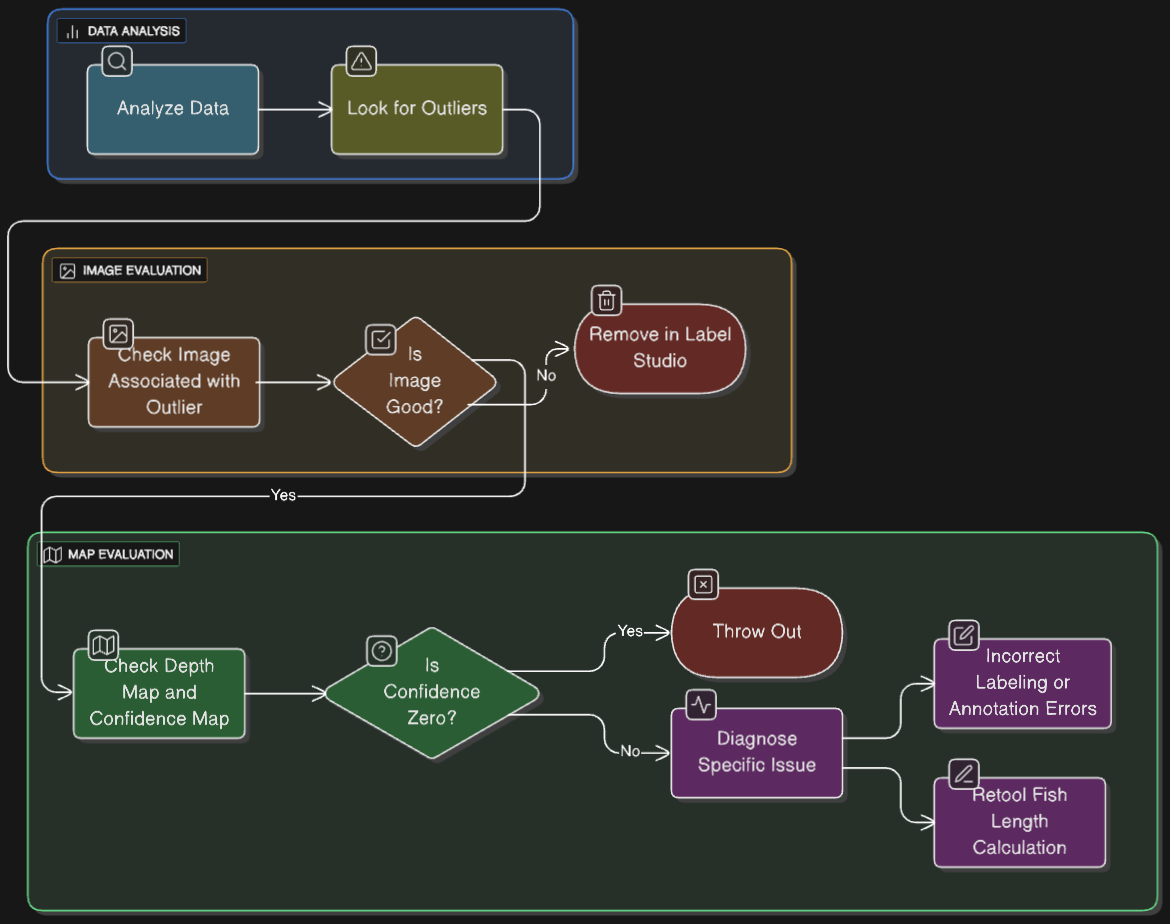
\includegraphics[width=\linewidth]{images/data_flowchart.png}
        \column{0.33\textwidth}
        \textbf{We found some pretty bad images}
        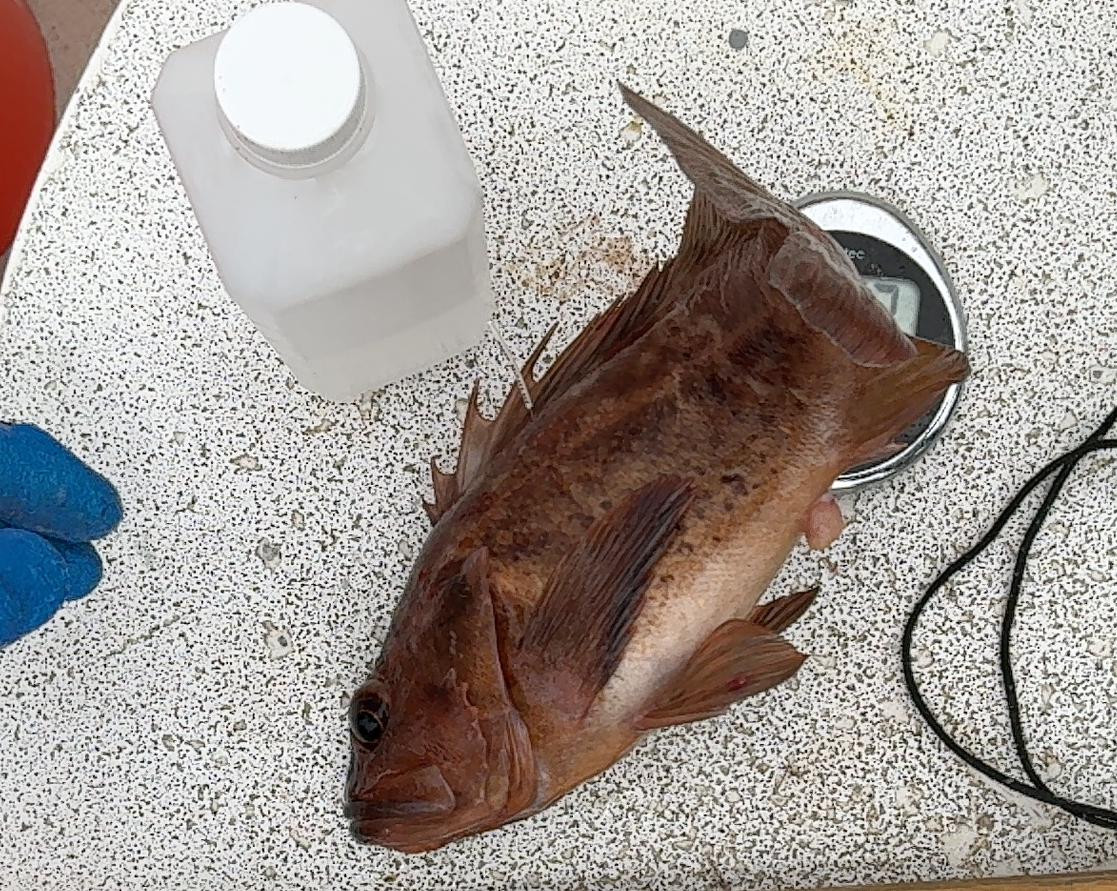
\includegraphics[width=\linewidth]{images/outlier.png}
    \end{columns}
\end{frame}


\begin{frame}{Problem: FishSense Mobile vs. FishTechy}
    \textbf{Lab Results}
    \begin{itemize}
        \item Consist of repeated images of the same fish
        \item Consistently poor performance for specific fish
        \item Possible explanations: fish is off-angle to plane, depth map "walks up" surfaces
    \end{itemize}
\end{frame}

\begin{frame}{DWE Camera Mount}
    \centering
    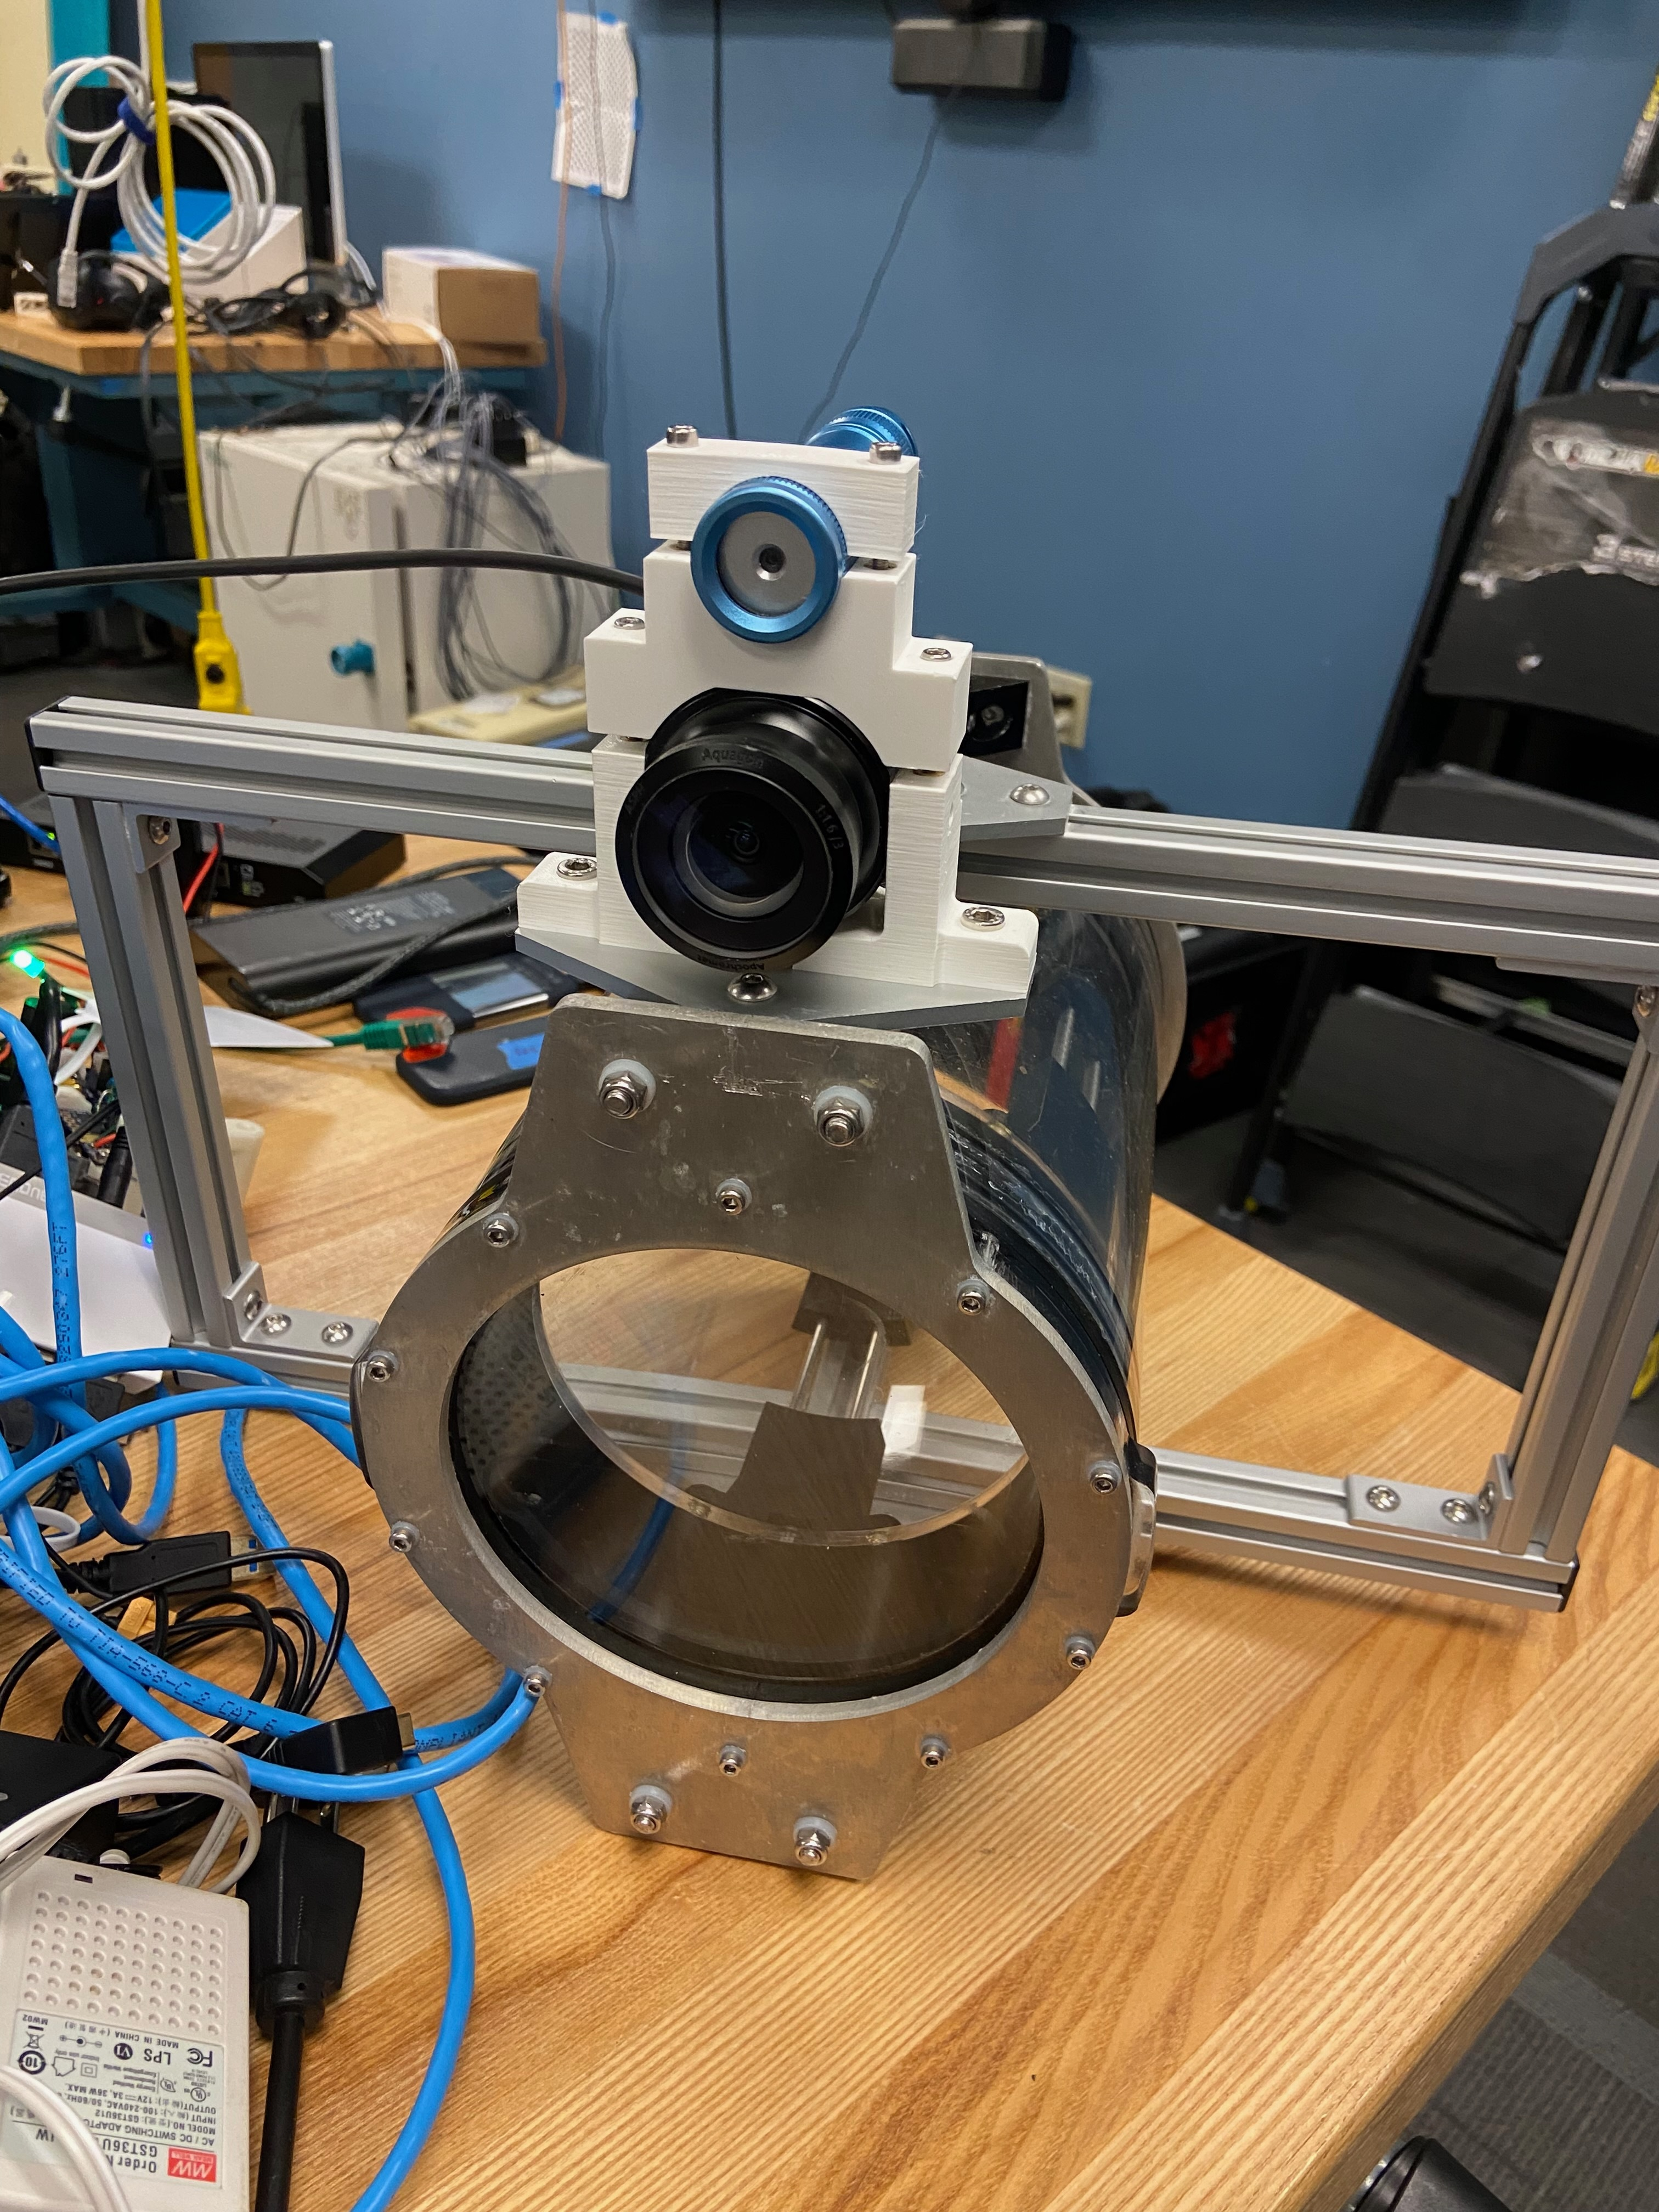
\includegraphics[height=0.7\textheight,width=0.7\textwidth,keepaspectratio]{images/dwe_camera_mounted_with_laser.jpeg}
\end{frame}

% pool testing
\begin{frame}{Pool Testing (with new camera!)}
    \begin{columns}[c]
        \column{0.33\textwidth}
        \centering
        
\includegraphics[width=\linewidth]{images/frame_00137.png}
        
        \column{0.33\textwidth}
        \centering
        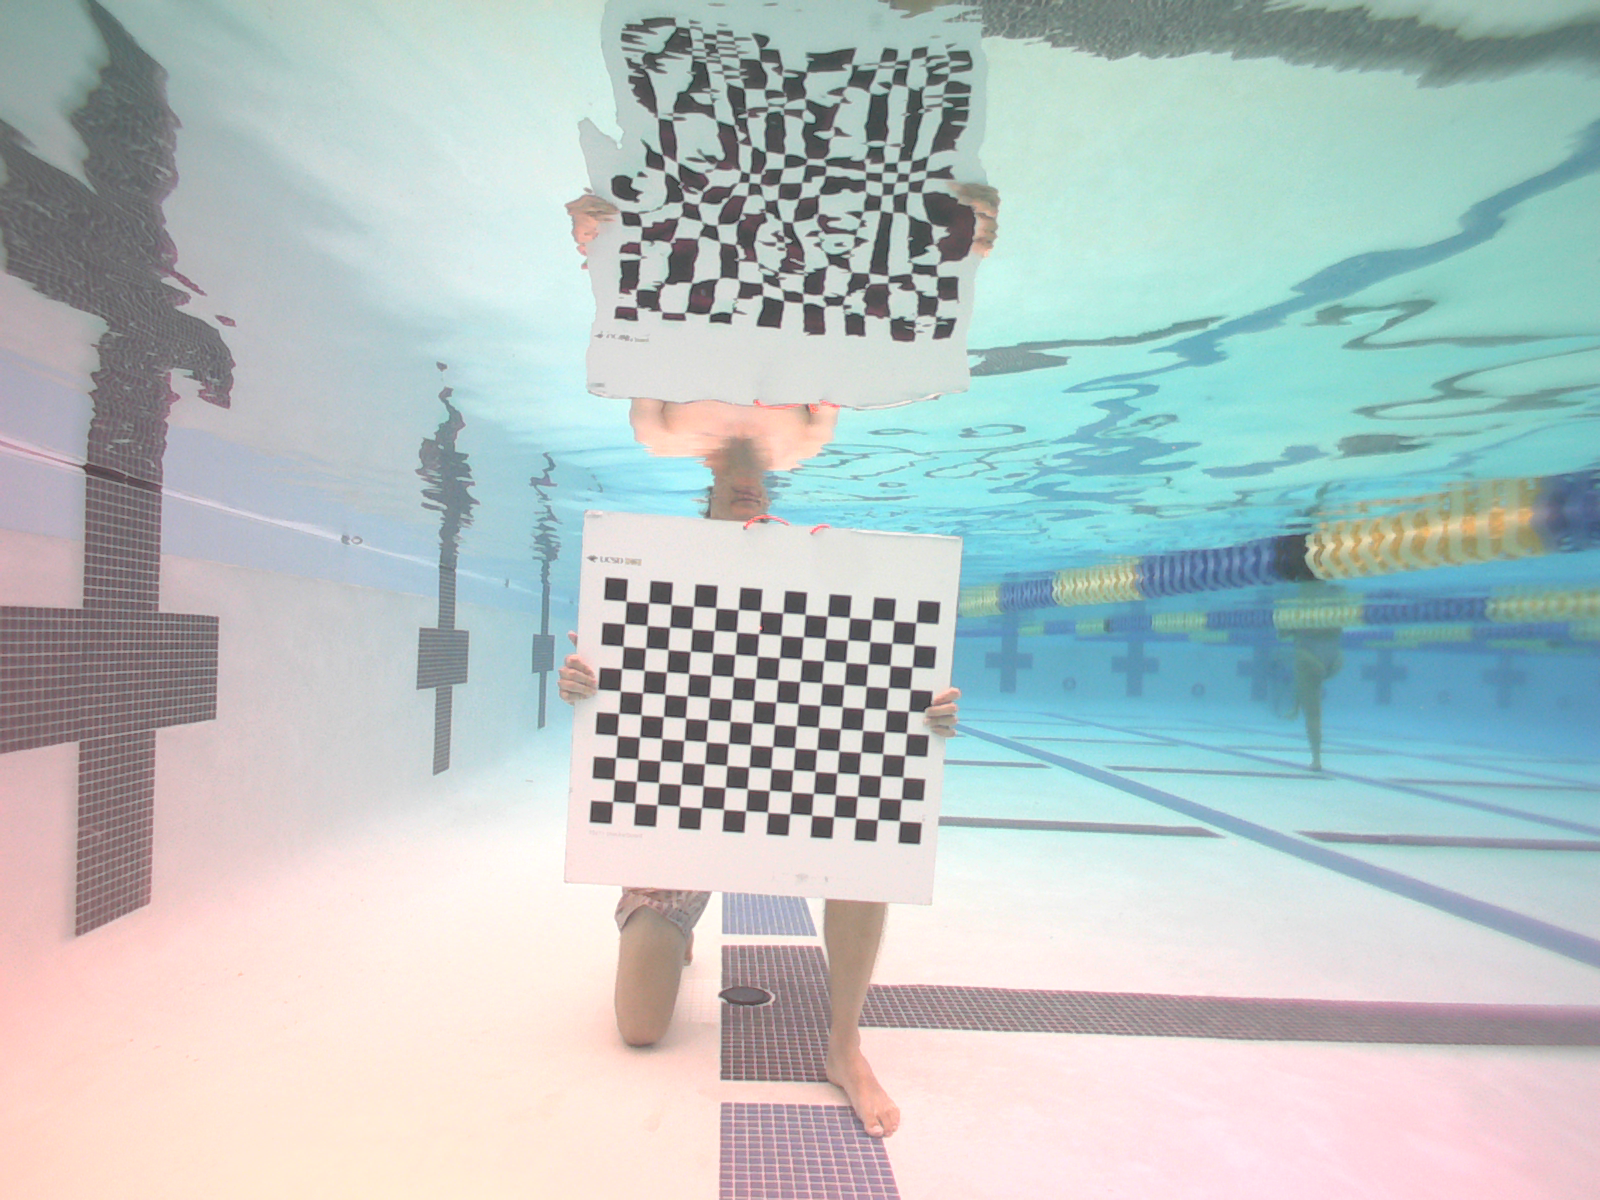
\includegraphics[width=\linewidth]{images/frame_02595.png}
        
        \column{0.33\textwidth}
        \centering
        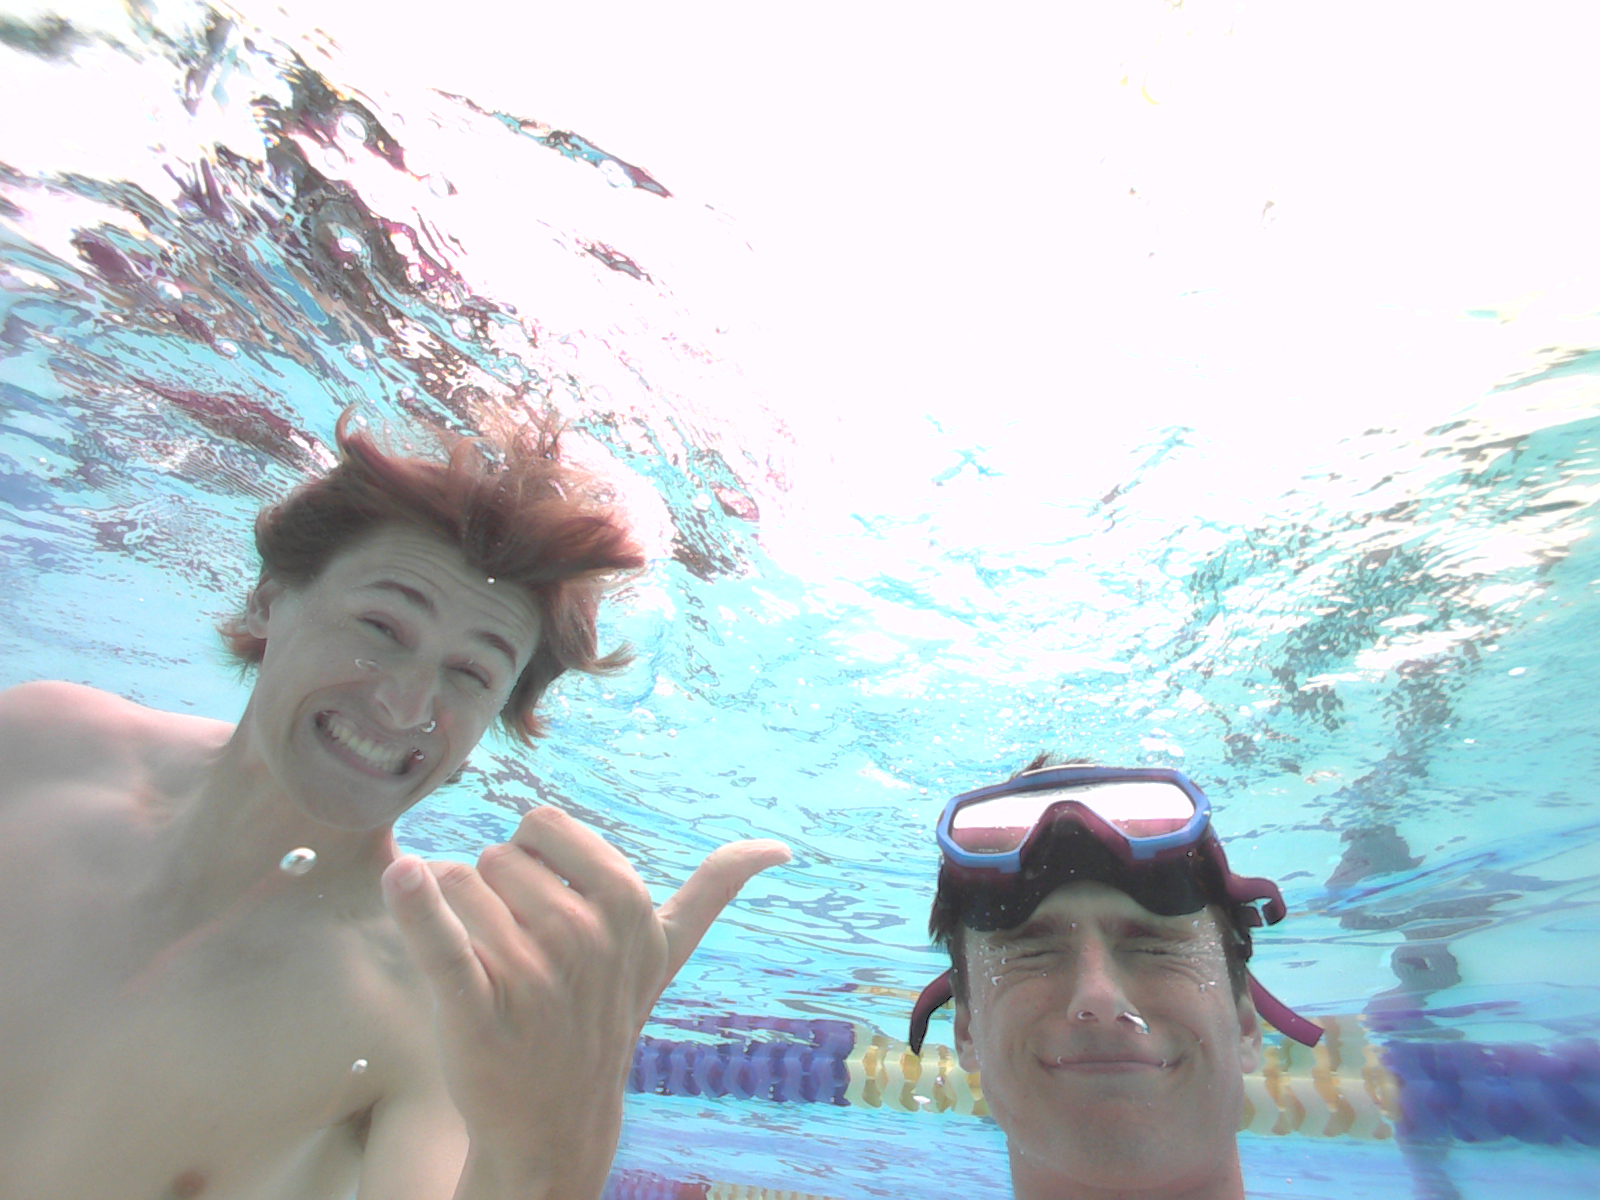
\includegraphics[width=\linewidth]{images/frame_02357.png}
    \end{columns}
\end{frame}

\begin{frame}{Breaking Bad}
    \centering
    \begin{tabular}{cc}
        \includegraphics[width=0.45\textwidth]{images/depthT_S04910.png} &
        \includegraphics[width=0.45\textwidth]{images/4910_corrected.png} \\
        \includegraphics[width=0.45\textwidth]{images/P7170010.png} &
        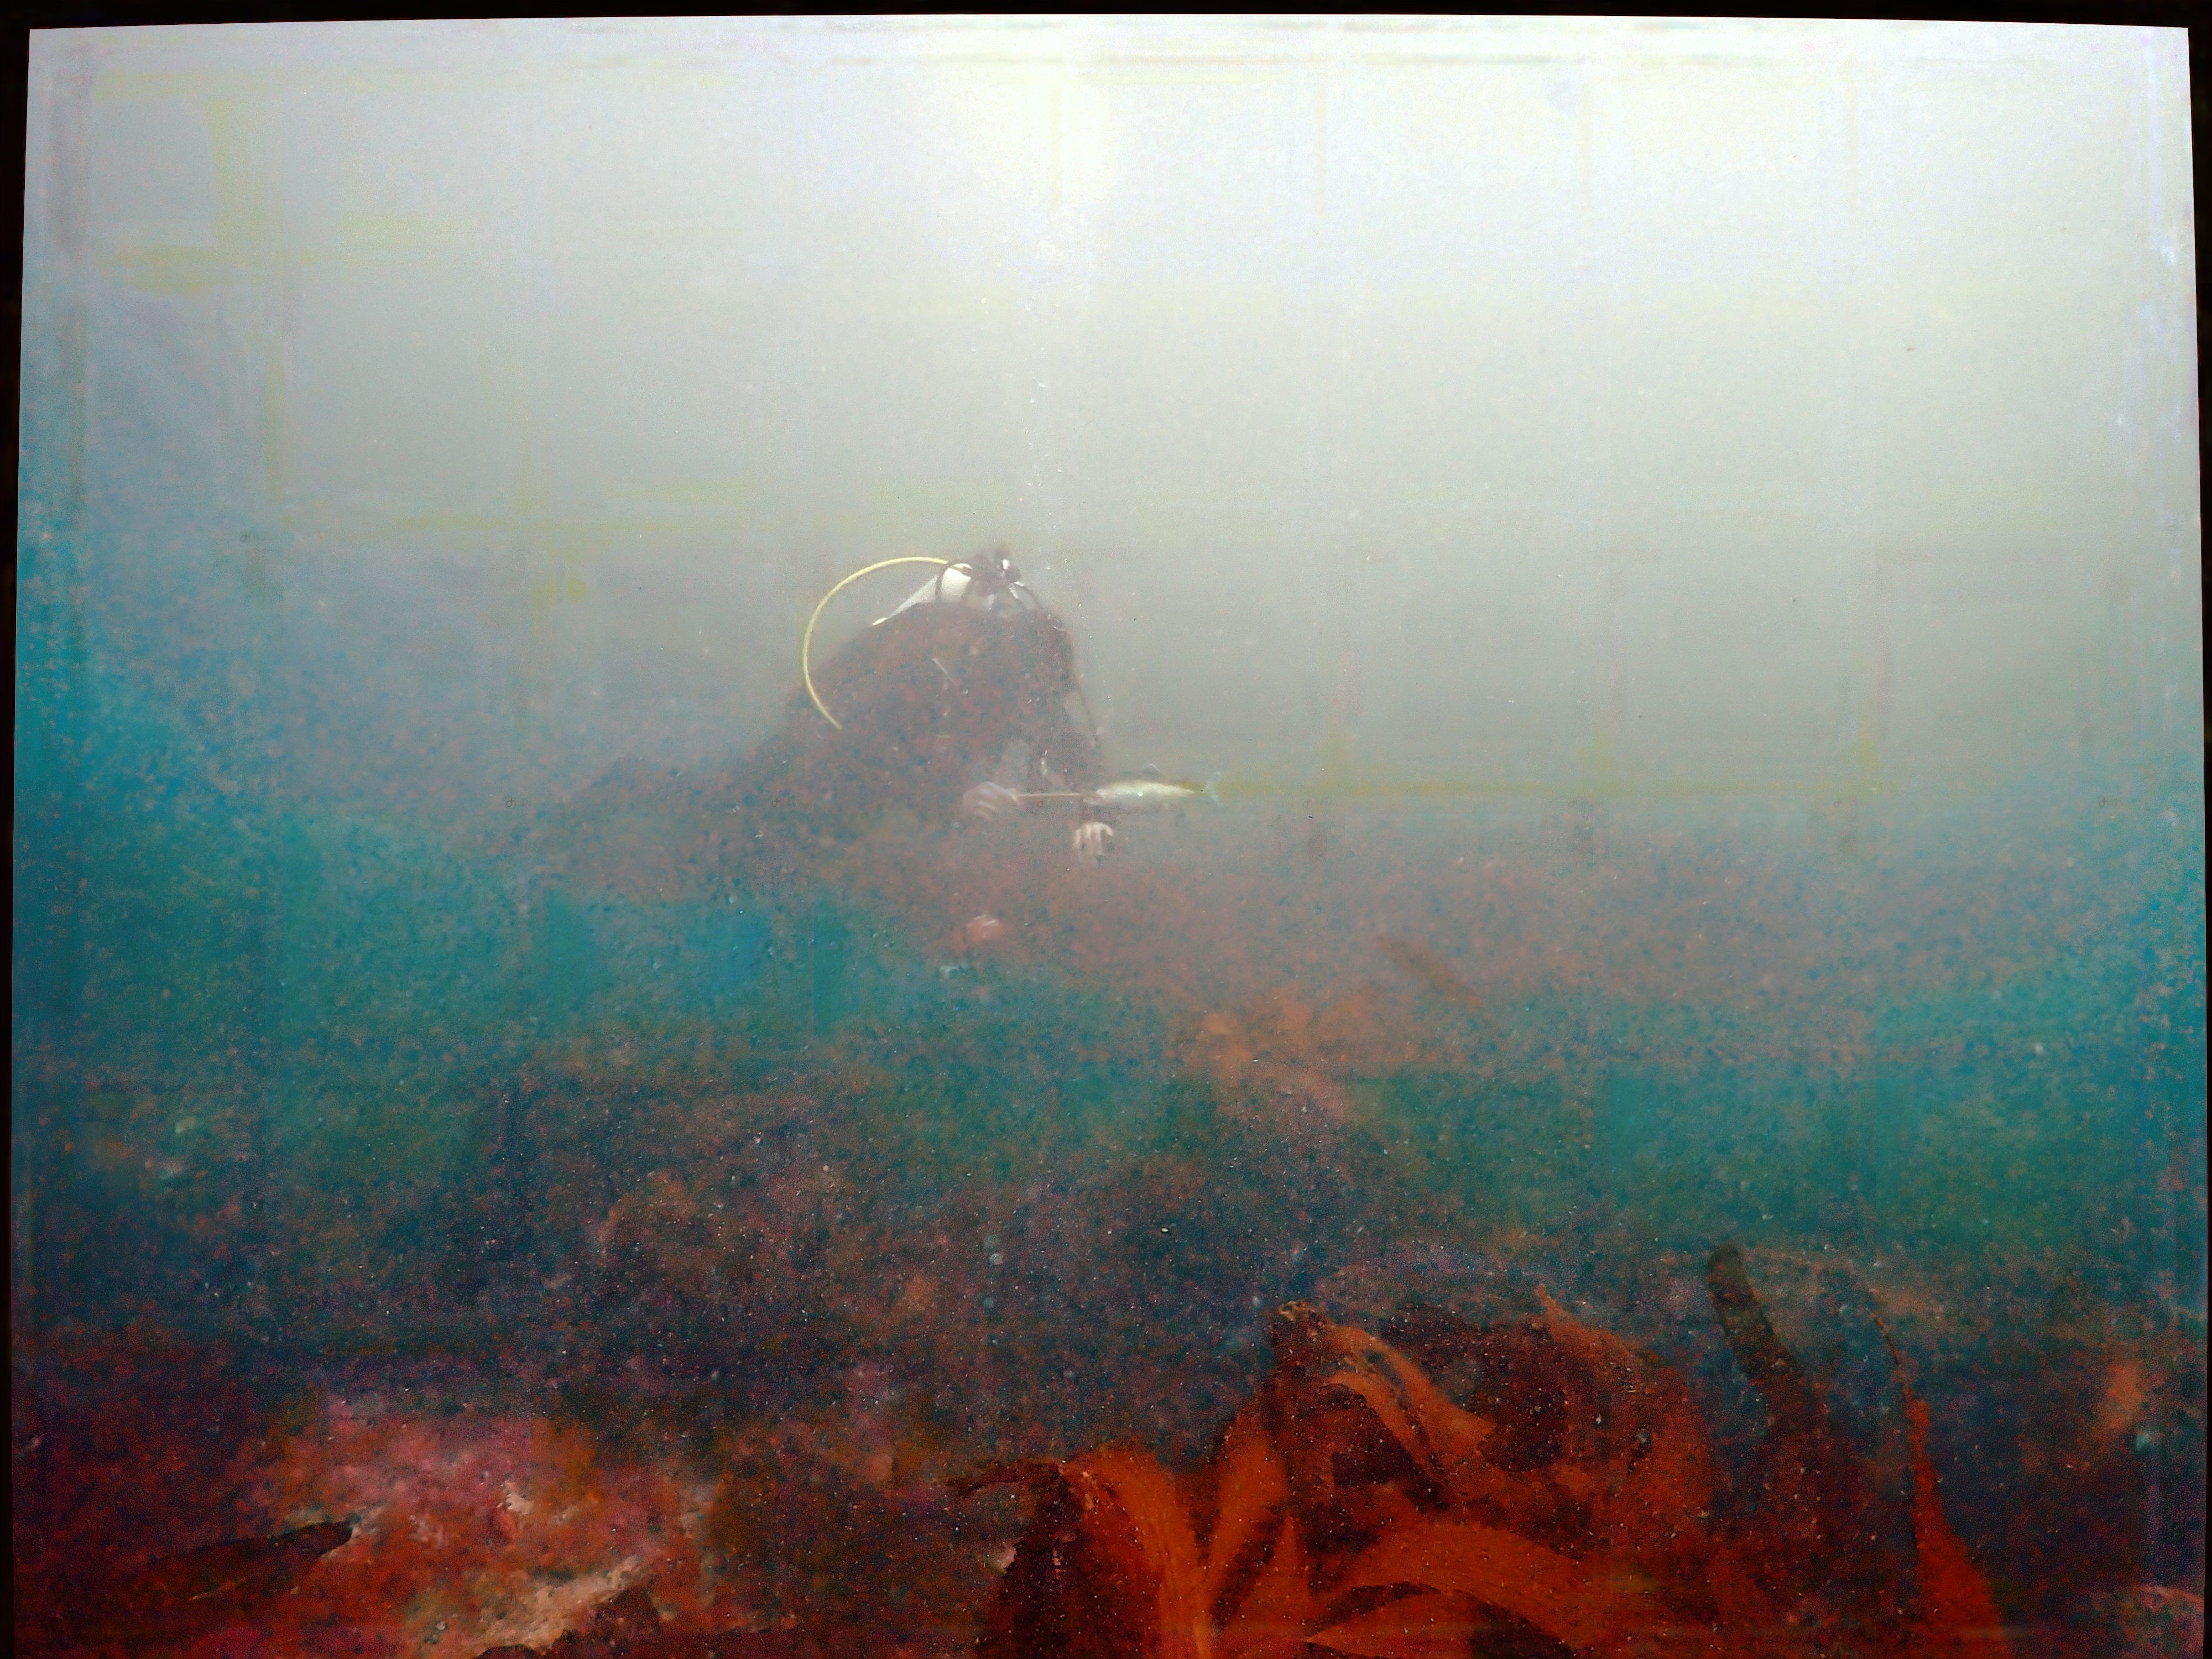
\includegraphics[width=0.45\textwidth]{images/P7170010_corrected.JPG} \\
    \end{tabular}
\end{frame}

% DO NOT DELETE MY SLIDE - BRENDON!!!!
\begin{frame}{FishSense Mobile Android}
    \vfill
    \centering
    \begin{columns}
        % Column 1: Camera Image
        \begin{column}{0.32\textwidth}
            \centering
            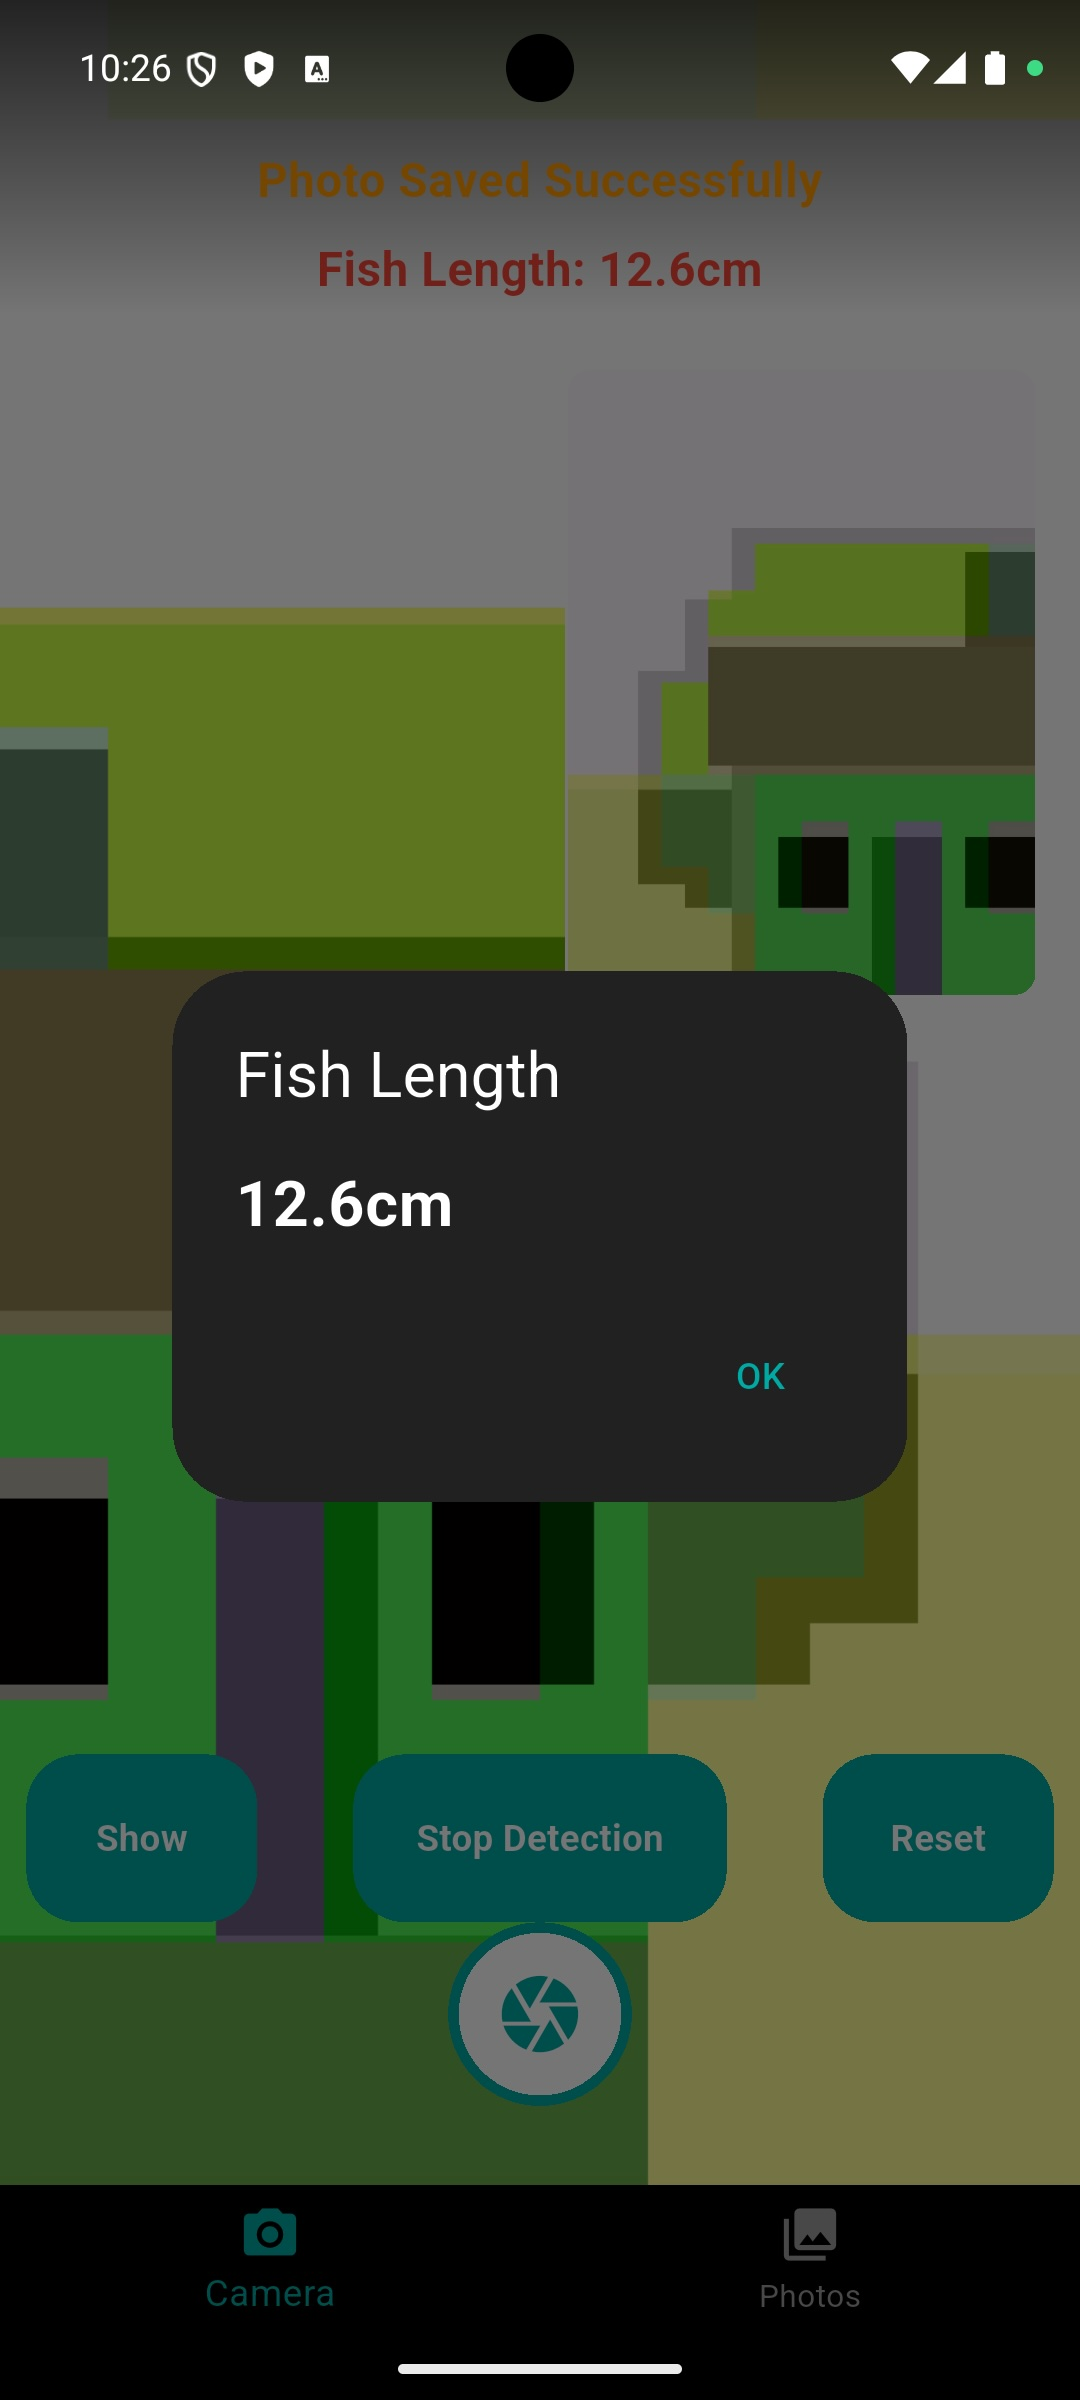
\includegraphics[height=0.8\textheight,keepaspectratio]{images/CameraImage.jpg}
            
            \vspace{0.2cm}
            \textbf{Current Progress:} \\
            Camera with Mock Data
        \end{column}
        
        % Column 2: Gallery Image
        \begin{column}{0.32\textwidth}
            \centering
            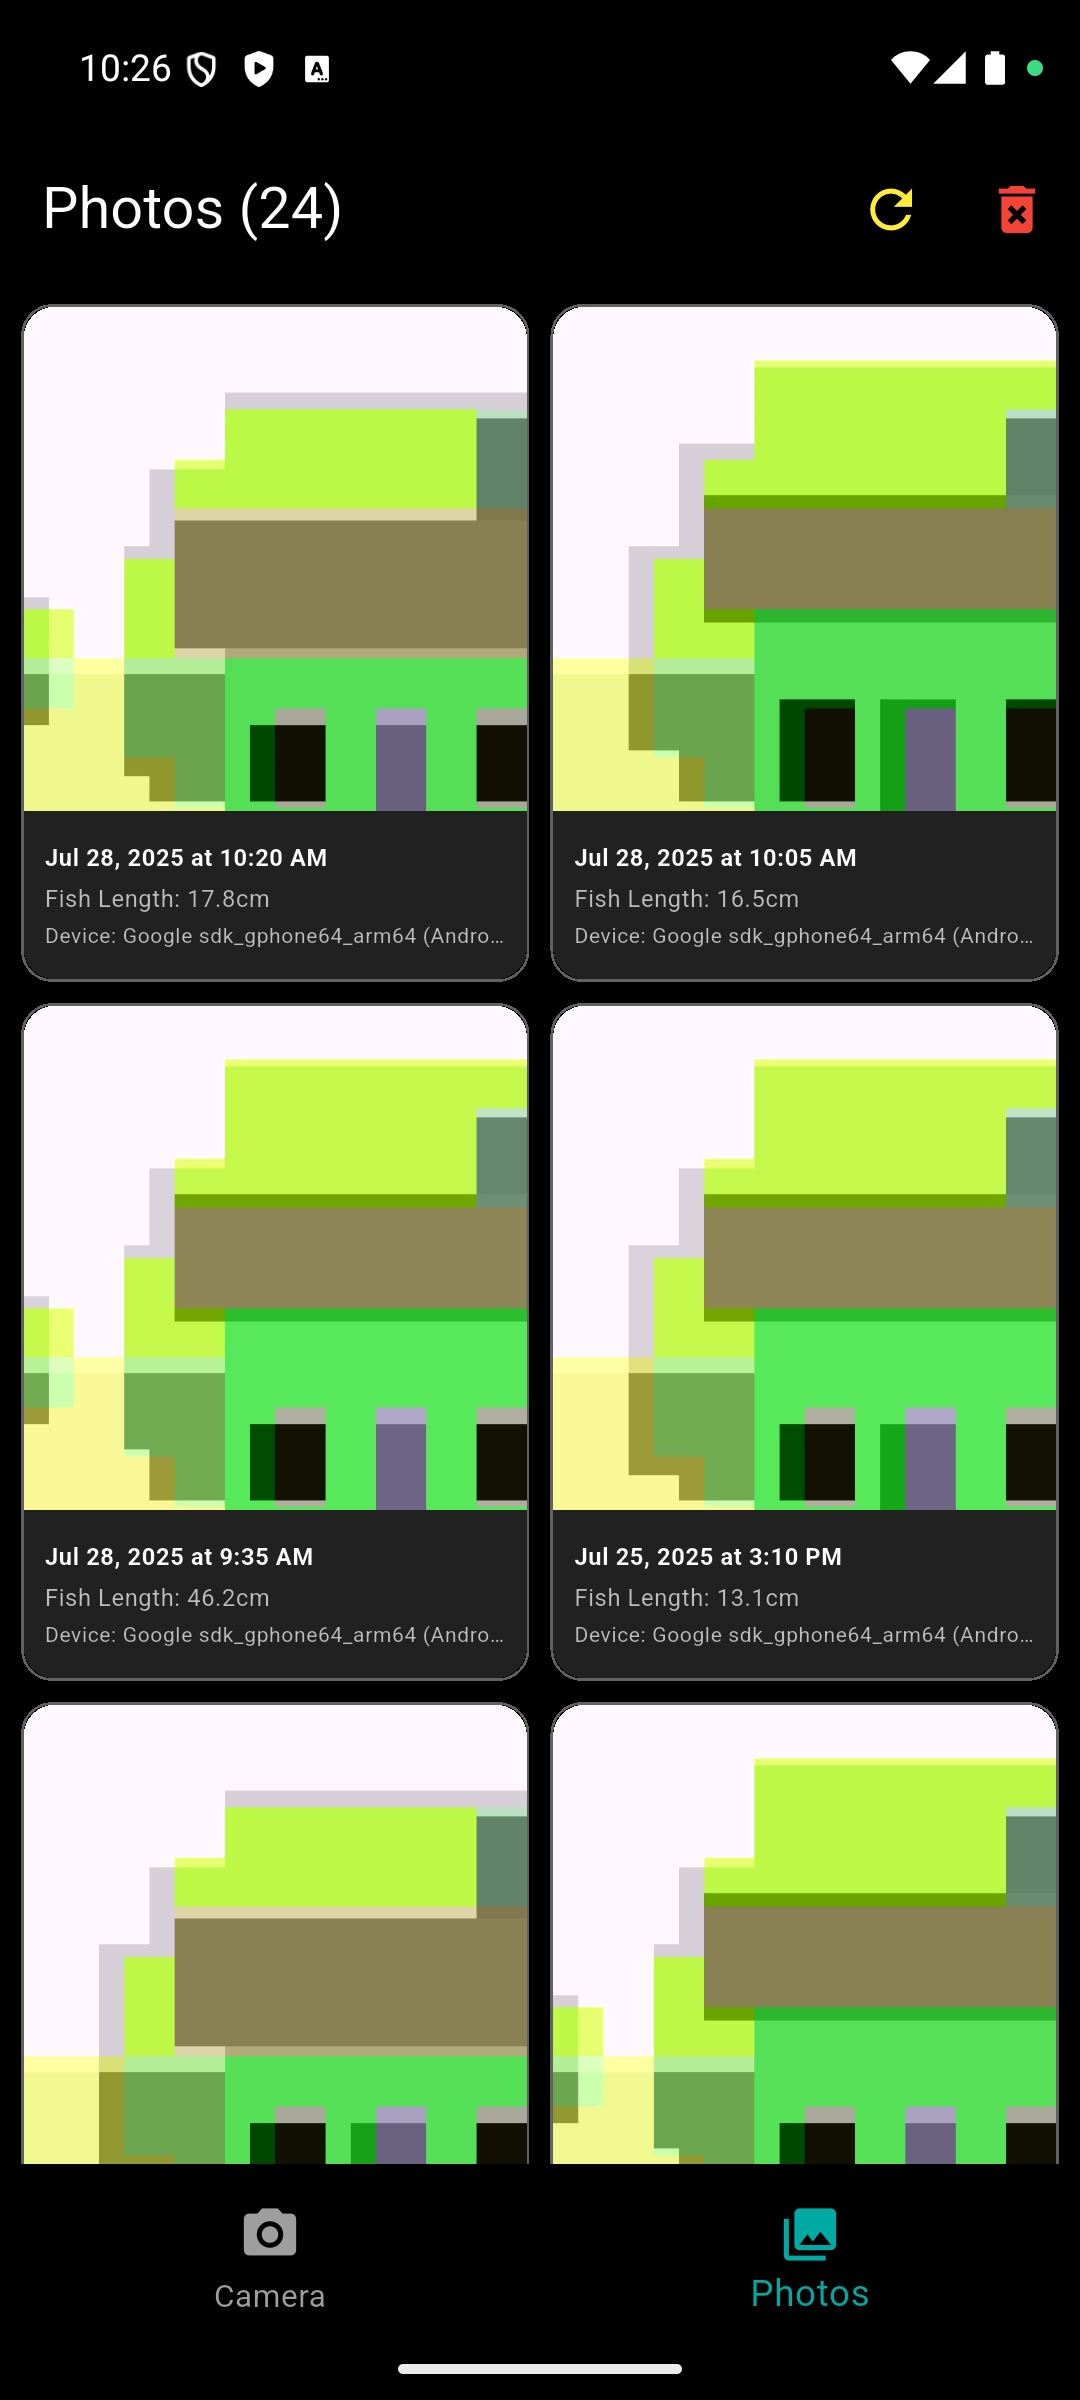
\includegraphics[height=0.8\textheight,keepaspectratio]{images/GalleryImage.jpg}
            
            \vspace{0.2cm}
            \textbf{Current Progress:} \\
            Gallery with Mock Data
        \end{column}
        
        % Column 3: Diagram Image
        \begin{column}{0.32\textwidth}
            \centering
            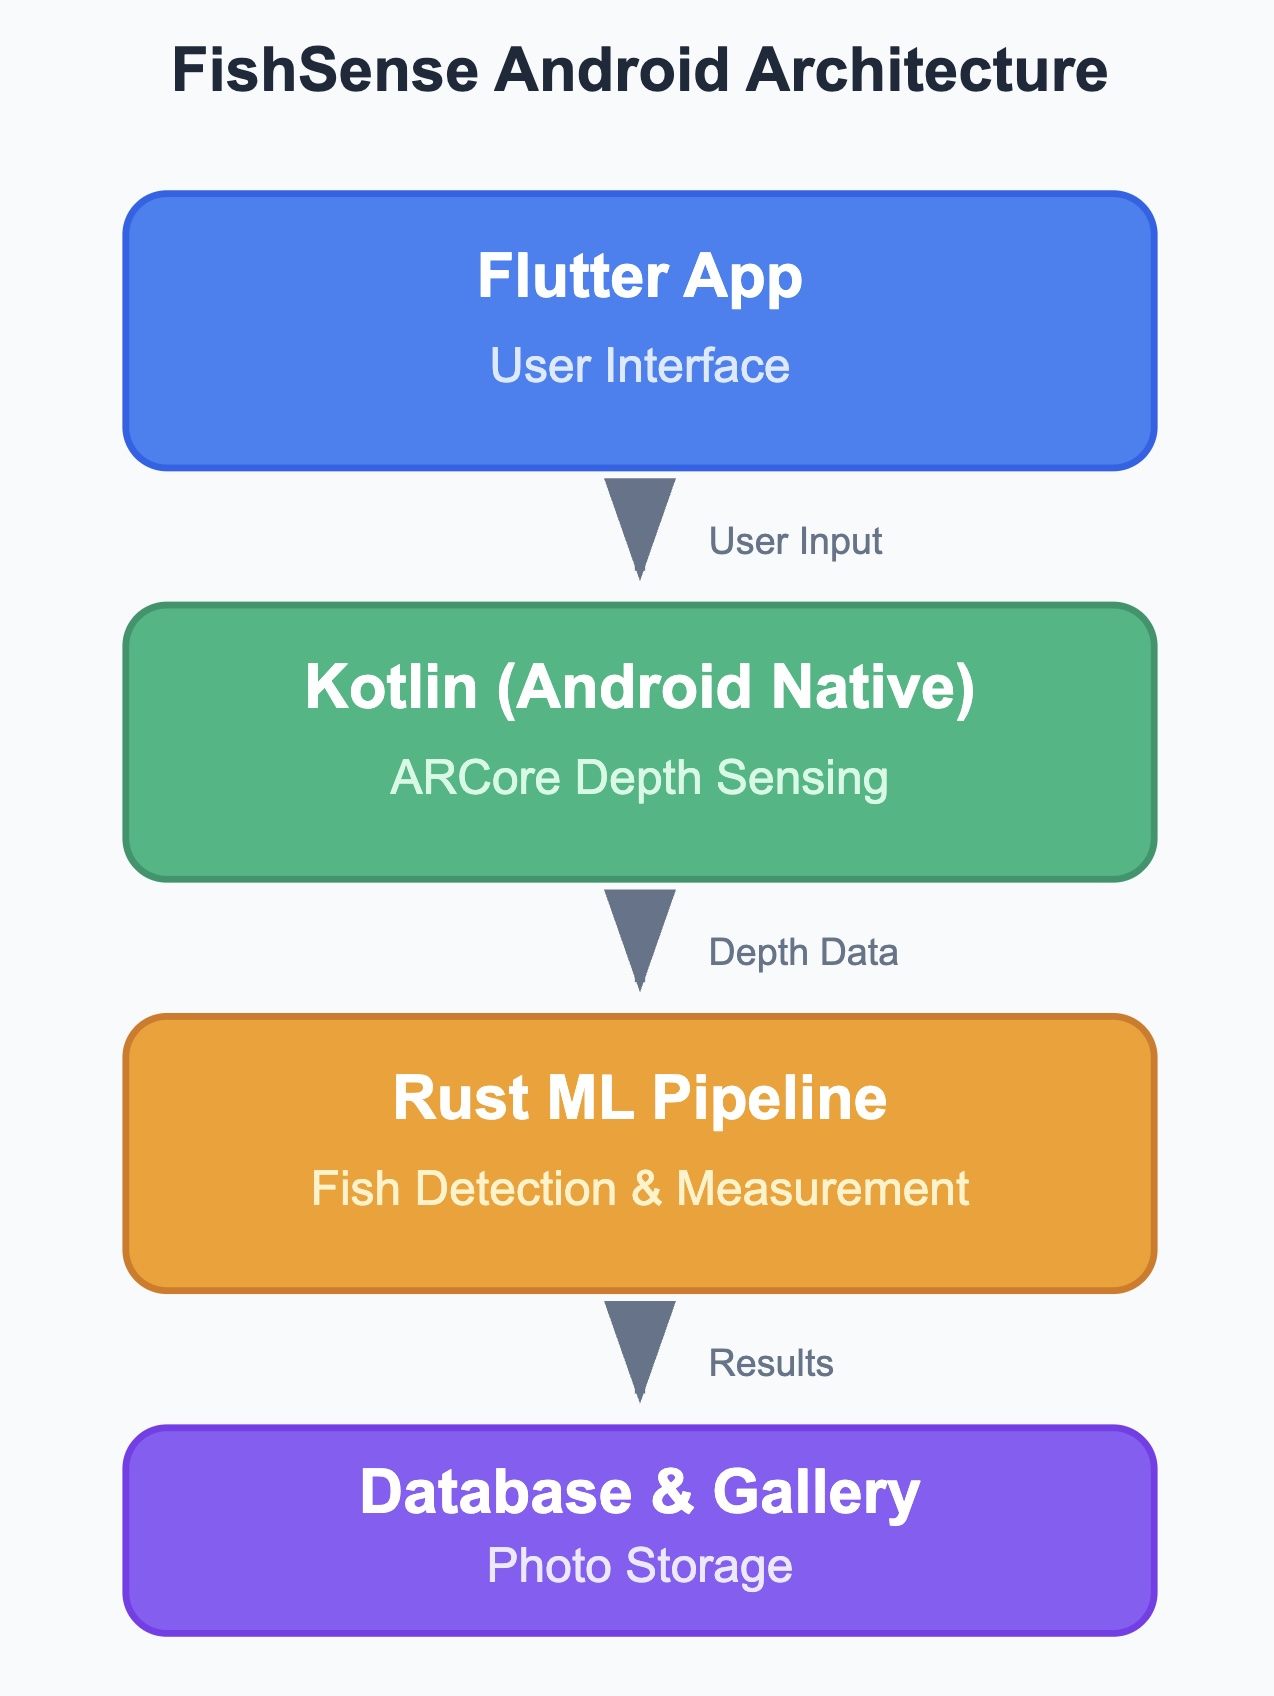
\includegraphics[height=0.7\textheight,keepaspectratio]{images/Diagram1.jpg}
            
            \vspace{0.1cm}
            \textbf{Next Steps:} \\
            ARCore Integration
        \end{column}
    \end{columns}
    \vfill
\end{frame}

